\documentclass[conference]{IEEEtran}

% Packages for publication-quality diagrams
\usepackage[utf8]{inputenc}
\usepackage{cite}
\usepackage{amsmath,amssymb,amsfonts}
\usepackage{algorithmic}
\usepackage{graphicx}
\usepackage{textcomp}
\usepackage{xcolor}
\usepackage{tikz}
\usetikzlibrary{shapes.geometric, arrows.meta, positioning, fit, calc, backgrounds, patterns, decorations.pathreplacing, shapes.multipart}
\usepackage{pgfplots}
\pgfplotsset{compat=1.17}
\usepackage{subcaption}
\usepackage{multirow}
\usepackage{booktabs}

% Define publication color scheme (grayscale-friendly)
\definecolor{blockfill}{RGB}{240,240,240}
\definecolor{emphasisfill}{RGB}{200,200,200}
\definecolor{signalcolor}{RGB}{80,80,80}
\definecolor{accentcolor}{RGB}{100,100,100}

% TikZ styles for publication diagrams
\tikzset{
    block/.style={
        rectangle,
        draw=black,
        thick,
        fill=blockfill,
        text centered,
        minimum height=2em,
        font=\footnotesize\sffamily
    },
    emphblock/.style={
        block,
        fill=emphasisfill,
        font=\footnotesize\sffamily\bfseries
    },
    smallblock/.style={
        block,
        minimum height=1.5em,
        font=\scriptsize\sffamily
    },
    dspblock/.style={
        block,
        minimum width=2.5cm,
        minimum height=1.2cm
    },
    connection/.style={
        draw=black,
        thick,
        -Stealth
    },
    bus/.style={
        draw=black,
        very thick,
        -Stealth
    },
    controlsignal/.style={
        draw=black,
        dashed,
        -Stealth
    },
    label/.style={
        font=\scriptsize\sffamily
    },
    statenode/.style={
        circle,
        draw=black,
        thick,
        fill=blockfill,
        text centered,
        minimum size=1.5cm,
        font=\scriptsize\sffamily
    }
}

\begin{document}

\title{AES-128 FPGA Implementation:\\Architecture and Design}

\author{\IEEEauthorblockN{Technical Documentation}
\IEEEauthorblockA{Hardware Security Implementation}}

\maketitle

%==============================================================================
% Figure 1: High-Level System Architecture
%==============================================================================
\begin{figure*}[t]
\centering
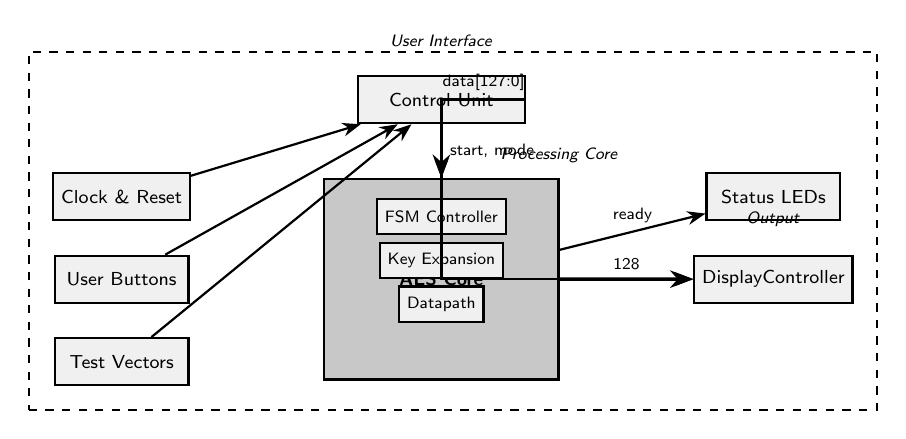
\begin{tikzpicture}[node distance=1.2cm and 1.5cm, scale=0.85, transform shape]

% Input interface
\node[block, minimum width=2cm] (clk_rst) {Clock \& Reset};
\node[block, minimum width=2cm, below=0.5cm of clk_rst] (buttons) {User Buttons};
\node[block, minimum width=2cm, below=0.5cm of buttons] (switches) {Test Vectors};

% Main processing blocks
\node[emphblock, minimum width=3.5cm, minimum height=3cm, right=2cm of buttons] (core) {AES Core};
\node[smallblock, below=0.3cm of core.north] (fsm) {FSM Controller};
\node[smallblock, below=0.1cm of fsm] (keyexp) {Key Expansion};
\node[smallblock, below=0.1cm of keyexp] (datapath) {Datapath};

% Control unit
\node[block, minimum width=2.5cm, above=0.8cm of core] (control) {Control Unit};

% Output interface
\node[block, minimum width=2cm, right=2cm of core] (display) {Display\\Controller};
\node[block, minimum width=2cm, above=0.5cm of display] (status) {Status LEDs};

% Connections
\draw[connection] (clk_rst) -- (control);
\draw[connection] (buttons) -- (control);
\draw[connection] (switches) -- (control);
\draw[connection] (control) -- node[label, right] {start, mode} (core);
\draw[bus] (control.east) -| node[label, near start, above] {data[127:0]} (core.north);
\draw[connection] (core) -- node[label, above] {ready} (status);
\draw[bus] (core) -- node[label, above] {128} (display);
\draw[connection] (control) |- (display);

% Annotations
\node[label, above=0.3cm of control] {\textit{User Interface}};
\node[label, above=0.1cm of core.north east] {\textit{Processing Core}};
\node[label, above=0.3cm of display] {\textit{Output}};

% Bounding box
\begin{scope}[on background layer]
\node[draw=black, thick, dashed, fit=(clk_rst) (buttons) (switches) (control) (core) (display) (status), inner sep=0.3cm] {};
\end{scope}

\end{tikzpicture}
\caption{High-level system architecture showing the main functional blocks and data flow. The AES core processes 128-bit blocks under FSM control, with user interface and display subsystems.}
\label{fig:system_arch}
\end{figure*}

%==============================================================================
% Figure 2: AES Core Architecture
%==============================================================================
\begin{figure*}[t]
\centering
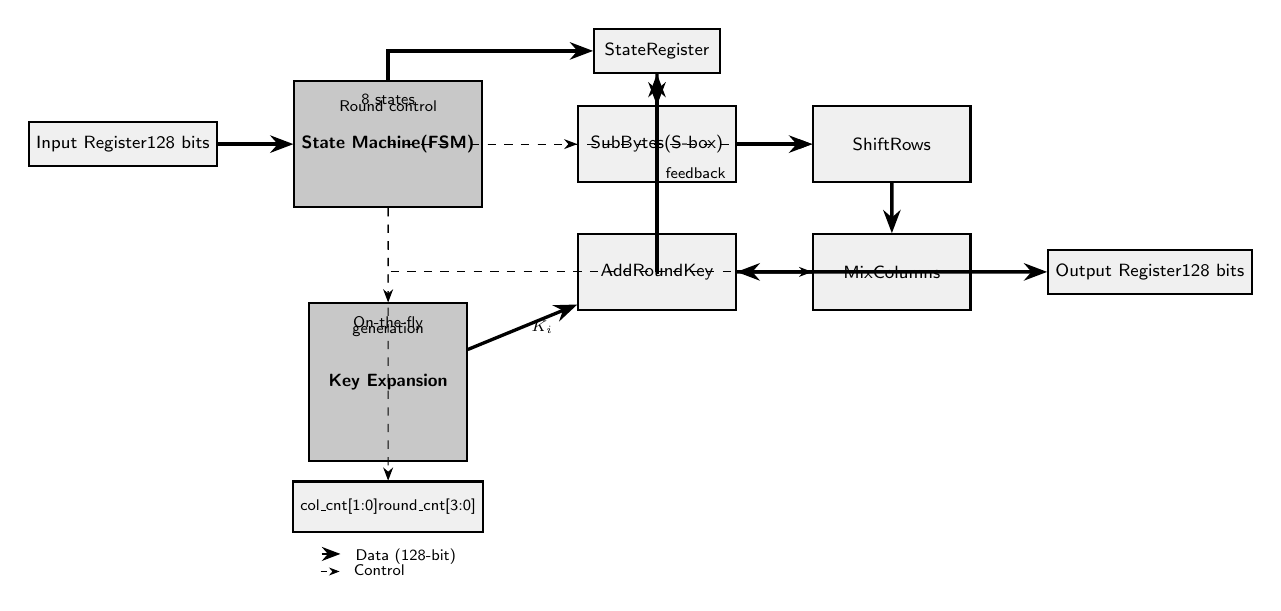
\begin{tikzpicture}[node distance=1cm and 1.2cm, scale=0.8, transform shape]

% Input registers
\node[block, minimum width=2.5cm] (input_reg) {Input Register\\128 bits};

% State machine
\node[emphblock, minimum width=2.5cm, minimum height=2cm, right=of input_reg] (fsm) {State Machine\\(FSM)};
\node[label, below=0.1cm of fsm.north] {\scriptsize 8 states};
\node[label, below=0.2cm of fsm.north] {\scriptsize Round control};

% Datapath components
\node[dspblock, right=1.5cm of fsm] (subbytes) {SubBytes\\(S-box)};
\node[dspblock, right=of subbytes] (shiftrows) {ShiftRows};
\node[dspblock, below=0.8cm of shiftrows] (mixcols) {MixColumns};
\node[dspblock, below=0.8cm of subbytes] (addroundkey) {AddRoundKey};

% Key expansion
\node[emphblock, minimum width=2.5cm, minimum height=2.5cm, below=1.5cm of fsm] (keyexp) {Key Expansion};
\node[label, below=0.1cm of keyexp.north] {\scriptsize On-the-fly};
\node[label, below=0.2cm of keyexp.north] {\scriptsize generation};

% Output register
\node[block, minimum width=2.5cm, right=1.2cm of mixcols] (output_reg) {Output Register\\128 bits};

% State storage
\node[block, minimum width=2cm, above=0.5cm of subbytes] (state_reg) {State\\Register};

% Connections - Data path
\draw[bus] (input_reg) -- (fsm);
\draw[bus] (fsm) |- (state_reg);
\draw[bus] (state_reg) -- (subbytes);
\draw[bus] (subbytes) -- (shiftrows);
\draw[bus] (shiftrows) -- (mixcols);
\draw[bus] (mixcols) -- (addroundkey);
\draw[bus] (addroundkey) -| node[label, near end, right] {feedback} (state_reg);
\draw[bus] (addroundkey) -- (output_reg);

% Key connections
\draw[bus] (keyexp) -- node[label, right] {$K_i$} (addroundkey);
\draw[controlsignal] (fsm) -- (keyexp);

% Control signals
\draw[controlsignal] (fsm) |- (subbytes);
\draw[controlsignal] (fsm) |- (shiftrows);
\draw[controlsignal] (fsm) |- (mixcols);

% Column counter annotation
\node[block, minimum width=1.5cm, minimum height=0.8cm, below=0.3cm of keyexp] (counter) {\scriptsize col\_cnt[1:0]\\[-0.1cm]\scriptsize round\_cnt[3:0]};
\draw[controlsignal] (fsm) -- (counter);

% Legend
\node[label, below=0.1cm of counter, align=left] {
\tikz{\draw[bus] (0,0) -- (0.3,0);} \, Data (128-bit)\\[-0.05cm]
\tikz{\draw[controlsignal] (0,0) -- (0.3,0);} \, Control
};

\end{tikzpicture}
\caption{Detailed AES core architecture. The design employs column-wise processing (32 bits per cycle) to minimize resource utilization. Key expansion operates on-the-fly to reduce memory requirements by 90\%.}
\label{fig:core_arch}
\end{figure*}

%==============================================================================
% Figure 3: State Machine Diagram
%==============================================================================
\begin{figure}[t]
\centering
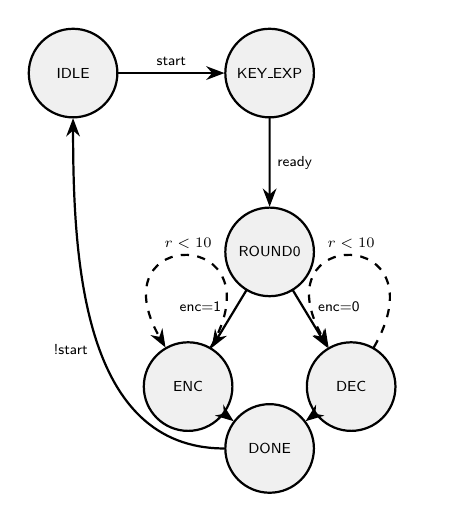
\begin{tikzpicture}[node distance=2.2cm, scale=0.75, transform shape]

% States
\node[statenode] (idle) {IDLE};
\node[statenode, right=1.8cm of idle] (keyexp) {KEY\_EXP};
\node[statenode, below=1.5cm of keyexp] (round0) {ROUND0};
\node[statenode, below left=1.2cm and 0.3cm of round0] (enc) {ENC};
\node[statenode, below right=1.2cm and 0.3cm of round0] (dec) {DEC};
\node[statenode, below=1.8cm of round0] (done) {DONE};

% Transitions
\draw[connection] (idle) -- node[label, above] {\scriptsize start} (keyexp);
\draw[connection] (keyexp) -- node[label, right] {\scriptsize ready} (round0);
\draw[connection] (round0) -- node[label, above left] {\scriptsize enc=1} (enc);
\draw[connection] (round0) -- node[label, above right] {\scriptsize enc=0} (dec);
\draw[connection] (enc) -- (done);
\draw[connection] (dec) -- (done);
\draw[connection] (done) to[out=180, in=270] node[label, below left] {\scriptsize !start} (idle);

% Round loop annotations
\draw[connection, dashed] (enc) to[out=60, in=120, looseness=8] node[label, above] {\scriptsize $r<10$} (enc);
\draw[connection, dashed] (dec) to[out=60, in=120, looseness=8] node[label, above] {\scriptsize $r<10$} (dec);

\end{tikzpicture}
\caption{FSM state diagram. After initial key expansion, the core performs 10 rounds of encryption or decryption operations, then asserts the ready signal.}
\label{fig:fsm}
\end{figure}

%==============================================================================
% Figure 4: Key Expansion Architecture
%==============================================================================
\begin{figure}[t]
\centering
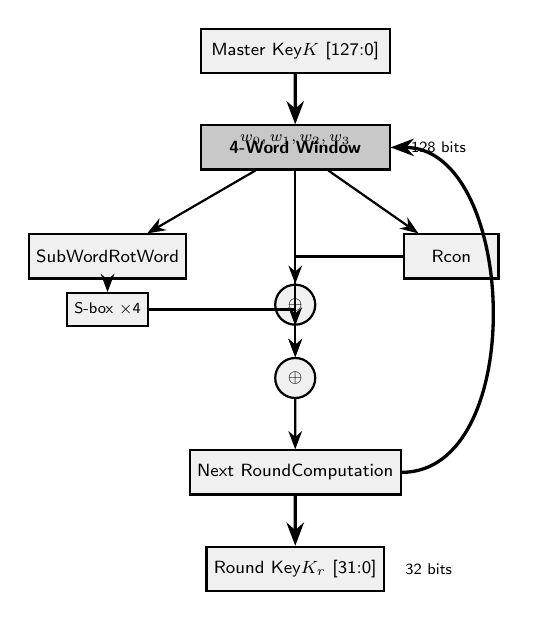
\begin{tikzpicture}[node distance=0.8cm and 1cm, scale=0.8, transform shape]

% Master key
\node[block, minimum width=3cm] (master) {Master Key\\$K$ [127:0]};

% Current window
\node[emphblock, minimum width=3cm, below=of master] (window) {4-Word Window};
\node[label, below=0.05cm of window.north] {\scriptsize $w_0, w_1, w_2, w_3$};

% SubWord
\node[block, minimum width=2cm, below left=1cm and 0.2cm of window] (subword) {SubWord\\RotWord};
\node[smallblock, below=0.2cm of subword] (sbox) {S-box $\times$4};

% Rcon
\node[block, minimum width=1.5cm, below right=1cm and 0.2cm of window] (rcon) {Rcon};

% XOR operation
\node[block, circle, minimum size=0.6cm, below=1.8cm of window] (xor1) {$\oplus$};
\node[block, circle, minimum size=0.6cm, below=0.5cm of xor1] (xor2) {$\oplus$};

% Next generation
\node[block, minimum width=2.5cm, below=0.8cm of xor2] (nextgen) {Next Round\\Computation};

% Output
\node[block, minimum width=2cm, below=of nextgen] (output) {Round Key\\$K_r$ [31:0]};

% Connections
\draw[bus] (master) -- (window);
\draw[connection] (window) -- (subword);
\draw[connection] (window) -- (rcon);
\draw[connection] (subword) -- (sbox);
\draw[connection] (sbox) -| (xor1);
\draw[connection] (window.south) -- ++(0,-0.5) -| (xor1);
\draw[connection] (rcon) -| (xor2);
\draw[connection] (xor1) -- (xor2);
\draw[connection] (xor2) -- (nextgen);
\draw[bus] (nextgen) to[out=0, in=0] (window);
\draw[bus] (nextgen) -- (output);

% Annotation
\node[label, right=0.2cm of window] {128 bits};
\node[label, right=0.2cm of output] {32 bits};

\end{tikzpicture}
\caption{On-the-fly key expansion architecture. Only the current 4-word window is stored (128 bits), achieving 90.9\% memory reduction compared to pre-computed approaches (1408 bits).}
\label{fig:keyexp}
\end{figure}

%==============================================================================
% Figure 5: Datapath Processing
%==============================================================================
\begin{figure}[t]
\centering
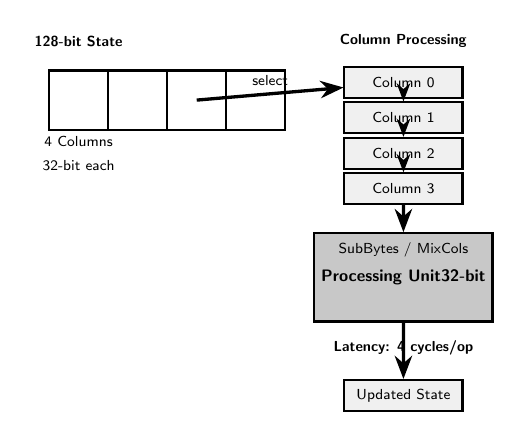
\begin{tikzpicture}[node distance=0.7cm, scale=0.75, transform shape]

% State matrix representation
\node[label] at (-2.5, 2) {\textbf{128-bit State}};
\draw[thick] (-3,1.5) rectangle (-2,0.5);
\draw[thick] (-2,1.5) rectangle (-1,0.5);
\draw[thick] (-1,1.5) rectangle (0,0.5);
\draw[thick] (0,1.5) rectangle (1,0.5);

\node[label] at (-2.5, 0.3) {4 Columns};
\node[label] at (-2.5, -0.1) {32-bit each};

% Sequential processing
\node[label] at (3, 2) {\textbf{Column Processing}};
\node[smallblock, minimum width=2cm] (col0) at (3, 1.3) {Column 0};
\node[smallblock, minimum width=2cm] (col1) at (3, 0.7) {Column 1};
\node[smallblock, minimum width=2cm] (col2) at (3, 0.1) {Column 2};
\node[smallblock, minimum width=2cm] (col3) at (3, -0.5) {Column 3};

\draw[connection] (col0) -- (col1);
\draw[connection] (col1) -- (col2);
\draw[connection] (col2) -- (col3);

% Processing unit
\node[emphblock, minimum width=2.5cm, minimum height=1.5cm] (pu) at (3, -2) {Processing Unit\\32-bit};
\node[label, below=0.05cm of pu.north] {\scriptsize SubBytes / MixCols};

\draw[bus] (-0.5, 1) -- node[label, above] {select} (col0);
\draw[bus] (col3) -- (pu);

% Timing
\node[label] at (3, -3.2) {\textbf{Latency: 4 cycles/op}};

% Result
\node[smallblock, minimum width=2cm] (result) at (3, -4) {Updated State};
\draw[bus] (pu) -- (result);

\end{tikzpicture}
\caption{Column-wise datapath processing. The design processes one 32-bit column per cycle, reducing combinational logic by 75\% compared to fully parallel implementations.}
\label{fig:datapath}
\end{figure}

%==============================================================================
% Figure 6: Round Operations
%==============================================================================
\begin{figure*}[t]
\centering
\begin{subfigure}[b]{0.48\textwidth}
\centering
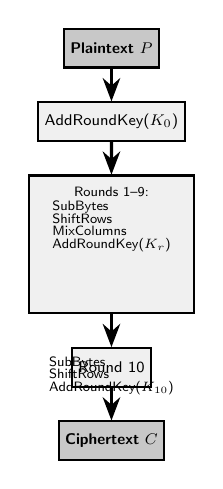
\begin{tikzpicture}[node distance=0.6cm, scale=0.7, transform shape]
% Encryption
\node[emphblock] (input) {Plaintext $P$};
\node[block, below=of input] (ark0) {AddRoundKey($K_0$)};
\node[block, below=of ark0, minimum height=2.5cm, minimum width=3cm] (rounds) {};
\node[label, below=0.1cm of rounds.north] {Rounds 1--9:};
\node[label, below=0.35cm of rounds.north, align=left] {\scriptsize SubBytes\\[-0.05cm]\scriptsize ShiftRows\\[-0.05cm]\scriptsize MixColumns\\[-0.05cm]\scriptsize AddRoundKey($K_r$)};
\node[block, below=of rounds] (round10) {Round 10};
\node[label, below=0.05cm of round10.north, align=left] {\scriptsize SubBytes\\[-0.05cm]\scriptsize ShiftRows\\[-0.05cm]\scriptsize AddRoundKey($K_{10}$)};
\node[emphblock, below=of round10] (output) {Ciphertext $C$};

\draw[bus] (input) -- (ark0);
\draw[bus] (ark0) -- (rounds);
\draw[bus] (rounds) -- (round10);
\draw[bus] (round10) -- (output);
\end{tikzpicture}
\caption{Encryption dataflow}
\end{subfigure}
\hfill
\begin{subfigure}[b]{0.48\textwidth}
\centering
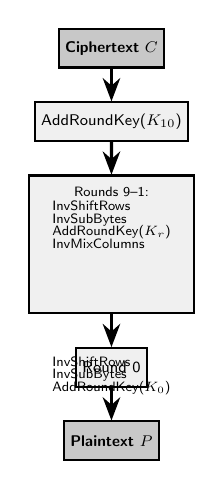
\begin{tikzpicture}[node distance=0.6cm, scale=0.7, transform shape]
% Decryption
\node[emphblock] (input) {Ciphertext $C$};
\node[block, below=of input] (ark0) {AddRoundKey($K_{10}$)};
\node[block, below=of ark0, minimum height=2.5cm, minimum width=3cm] (rounds) {};
\node[label, below=0.1cm of rounds.north] {Rounds 9--1:};
\node[label, below=0.35cm of rounds.north, align=left] {\scriptsize InvShiftRows\\[-0.05cm]\scriptsize InvSubBytes\\[-0.05cm]\scriptsize AddRoundKey($K_r$)\\[-0.05cm]\scriptsize InvMixColumns};
\node[block, below=of rounds] (round10) {Round 0};
\node[label, below=0.05cm of round10.north, align=left] {\scriptsize InvShiftRows\\[-0.05cm]\scriptsize InvSubBytes\\[-0.05cm]\scriptsize AddRoundKey($K_0$)};
\node[emphblock, below=of round10] (output) {Plaintext $P$};

\draw[bus] (input) -- (ark0);
\draw[bus] (ark0) -- (rounds);
\draw[bus] (rounds) -- (round10);
\draw[bus] (round10) -- (output);
\end{tikzpicture}
\caption{Decryption dataflow}
\end{subfigure}
\caption{Complete AES-128 encryption and decryption data flows. Note the symmetric structure with inverse operations in reverse order for decryption, and the absence of MixColumns/InvMixColumns in the final rounds.}
\label{fig:operations}
\end{figure*}

%==============================================================================
% Figure 7: Resource Utilization Chart
%==============================================================================
\begin{figure}[t]
\centering
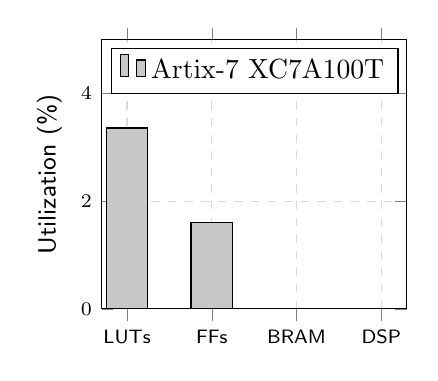
\begin{tikzpicture}
\begin{axis}[
    ybar,
    bar width=15pt,
    ylabel={Utilization (\%)},
    symbolic x coords={LUTs, FFs, BRAM, DSP},
    xtick=data,
    ymin=0, ymax=5,
    width=0.45\textwidth,
    height=5cm,
    legend pos=north west,
    grid=major,
    grid style={dashed, gray!30},
    ylabel style={font=\small\sffamily},
    xlabel style={font=\small\sffamily},
    tick label style={font=\scriptsize\sffamily}
]
\addplot[fill=emphasisfill, draw=black] coordinates {
    (LUTs, 3.36)
    (FFs, 1.61)
    (BRAM, 0)
    (DSP, 0)
};
\legend{Artix-7 XC7A100T}
\end{axis}
\end{tikzpicture}
\caption{FPGA resource utilization on Xilinx Artix-7. The design achieves very low resource usage through column-wise processing and on-the-fly key expansion, with no BRAM or DSP blocks required.}
\label{fig:resources}
\end{figure}

%==============================================================================
% Figure 8: Performance Comparison
%==============================================================================
\begin{figure}[t]
\centering
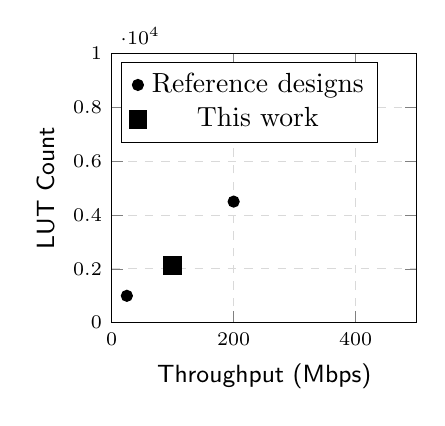
\begin{tikzpicture}
\begin{axis}[
    xlabel={Throughput (Mbps)},
    ylabel={LUT Count},
    xmin=0, xmax=500,
    ymin=0, ymax=10000,
    width=0.45\textwidth,
    height=5cm,
    grid=major,
    grid style={dashed, gray!30},
    legend pos=north west,
    xlabel style={font=\small\sffamily},
    ylabel style={font=\small\sffamily},
    tick label style={font=\scriptsize\sffamily}
]

% Data points
\addplot[only marks, mark=*, mark size=2pt, color=black] coordinates {
    (25, 1000)    % Serial
    (100, 2132)   % This work
    (200, 4500)   % Intermediate
    (400, 8000)   % Fully parallel
};

\addplot[only marks, mark=square*, mark size=3pt, color=black, thick] coordinates {
    (100, 2132)   % This work highlighted
};

\legend{Reference designs, This work}

\end{axis}
\end{tikzpicture}
\caption{Performance-area trade-off comparison. This work achieves balanced throughput (100 Mbps at 100 MHz) with significantly lower resource utilization compared to fully parallel implementations.}
\label{fig:performance}
\end{figure}

%==============================================================================
% Figure 9: Timing Diagram
%==============================================================================
\begin{figure*}[t]
\centering
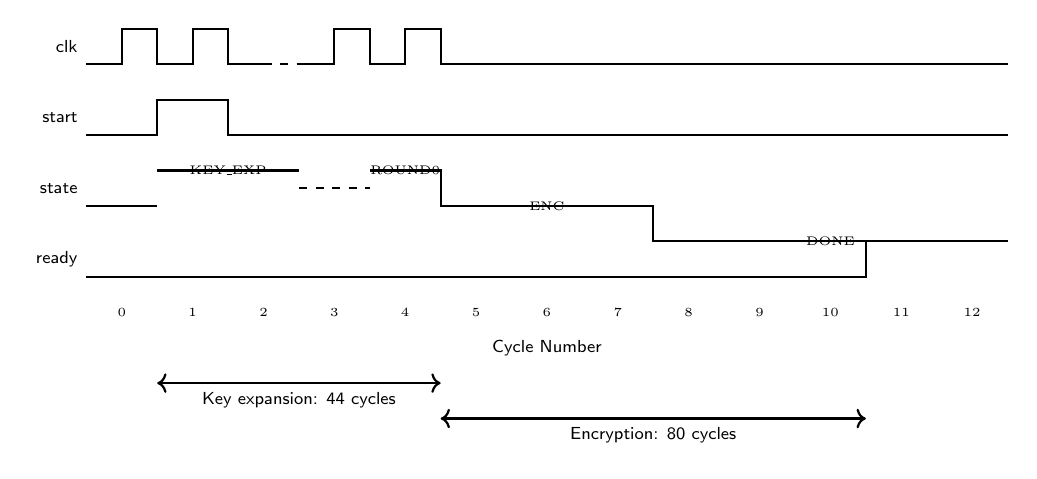
\begin{tikzpicture}[scale=0.9, transform shape]

% Clock
\draw[thick] (0,3) -- (0.5,3) -- (0.5,3.5) -- (1,3.5) -- (1,3) -- (1.5,3) -- (1.5,3.5) -- (2,3.5) -- (2,3) -- (2.5,3);
\draw[thick, dashed] (2.5,3) -- (3,3);
\draw[thick] (3,3) -- (3.5,3) -- (3.5,3.5) -- (4,3.5) -- (4,3) -- (4.5,3) -- (4.5,3.5) -- (5,3.5) -- (5,3) -- (13,3);
\node[label, left] at (0,3.25) {clk};

% Start signal
\draw[thick] (0,2) -- (1,2) -- (1,2.5) -- (2,2.5) -- (2,2) -- (13,2);
\node[label, left] at (0,2.25) {start};

% State signal
\draw[thick] (0,1) -- (1,1);
\draw[thick] (1,1.5) -- (3,1.5);
\draw[thick, dashed] (3,1.25) -- (4,1.25);
\draw[thick] (4,1.5) -- (5,1.5) -- (5,1) -- (8,1) -- (8,0.5) -- (13,0.5);
\node[label, left] at (0,1.25) {state};
\node[label, font=\tiny] at (2,1.5) {KEY\_EXP};
\node[label, font=\tiny] at (4.5,1.5) {ROUND0};
\node[label, font=\tiny] at (6.5,1) {ENC};
\node[label, font=\tiny] at (10.5,0.5) {DONE};

% Ready signal
\draw[thick] (0,0) -- (11,0) -- (11,0.5) -- (13,0.5);
\node[label, left] at (0,0.25) {ready};

% Cycle numbers
\foreach \x in {0,1,2,3,4,5,6,7,8,9,10,11,12} {
    \node[label, font=\tiny] at (\x+0.5,-0.5) {\x};
}
\node[label] at (6.5,-1) {Cycle Number};

% Annotations
\draw[<->, thick] (1,-1.5) -- (5,-1.5);
\node[label, below] at (3,-1.5) {Key expansion: 44 cycles};

\draw[<->, thick] (5,-2) -- (11,-2);
\node[label, below] at (8,-2) {Encryption: 80 cycles};

\end{tikzpicture}
\caption{Timing diagram showing a complete AES encryption operation. Total latency is 128 cycles (44 for key expansion + 4 for initial round + 72 for main rounds + 8 for final round), corresponding to 1.28~$\mu$s at 100~MHz.}
\label{fig:timing}
\end{figure*}

%==============================================================================
% Table: Implementation Comparison
%==============================================================================
\begin{table}[t]
\centering
\caption{Implementation Comparison with Related Work}
\label{tab:comparison}
\scriptsize
\begin{tabular}{@{}lccccc@{}}
\toprule
\textbf{Design} & \textbf{Device} & \textbf{LUTs} & \textbf{Freq.} & \textbf{Tput} & \textbf{Eff.} \\
 & & & \textbf{(MHz)} & \textbf{(Mbps)} & \textbf{(Mbps/LUT)} \\
\midrule
This work & Artix-7 & 2,132 & 100 & 100 & 0.047 \\
Serial [1] & Artix-7 & $\sim$1,000 & 100 & 25 & 0.025 \\
Parallel [2] & Artix-7 & $\sim$8,000 & 100 & 400 & 0.050 \\
Pipeline [3] & Virtex-7 & $\sim$15,000 & 250 & 3,200 & 0.213 \\
\bottomrule
\end{tabular}
\end{table}

%==============================================================================
% Table: Resource Breakdown
%==============================================================================
\begin{table}[t]
\centering
\caption{Detailed Resource Utilization Breakdown}
\label{tab:resources}
\scriptsize
\begin{tabular}{@{}lrrr@{}}
\toprule
\textbf{Resource Type} & \textbf{Used} & \textbf{Available} & \textbf{Util. (\%)} \\
\midrule
Slice LUTs & 2,132 & 63,400 & 3.36 \\
\quad LUT as Logic & 2,132 & 63,400 & 3.36 \\
\quad LUT as Memory & 0 & 19,000 & 0.00 \\
Slice Registers & 2,043 & 126,800 & 1.61 \\
\quad Flip-Flops & 2,043 & 126,800 & 1.61 \\
\quad Latches & 0 & 126,800 & 0.00 \\
F7 Muxes & 366 & 31,700 & 1.15 \\
F8 Muxes & 34 & 15,850 & 0.21 \\
Block RAM & 0 & 135 & 0.00 \\
DSP Slices & 0 & 240 & 0.00 \\
\midrule
\textbf{Total Power} & \multicolumn{3}{c}{\textbf{172 mW}} \\
\bottomrule
\end{tabular}
\end{table}

\end{document}
